\documentclass{standalone}
\usepackage{tikz}
\usepackage{ctex,siunitx}
\usepackage{tkz-euclide}
\usepackage{amsmath}
\usetikzlibrary{patterns, calc}
\usetikzlibrary {decorations.pathmorphing, decorations.pathreplacing, decorations.shapes,}
\begin{document}
\small
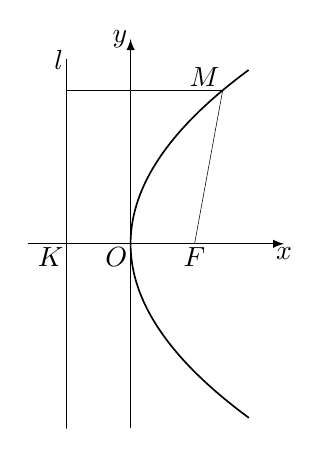
\begin{tikzpicture}[>=latex,scale=1.3,inner sep=1pt]
  \draw[thin,->](-1,0)--(1.5,0)node[below]{$x$};
  \draw[thin,->](0,-1.8)--(0,2.0)node[left]{$y$};
  \tkzDefPoints{0/0/O,0.625/0/F,-0.625/0/K,0.9/1.5/M,-0.625/1.5/P}
  \draw[semithick,domain=-1.7:1.7,samples=200] plot ({0.4*\x*\x},{\x});
  \tkzDrawSegments(M,P M,F)
  \tkzLabelPoints[above left](M)
  \tkzLabelPoints[below](F)
  \tkzDrawLine[semithick,add=0.2 and 1.2](P,K)
  \tkzLabelLine[pos=-0.2,left](P,K){$l$}
  \tkzLabelPoints[below left](O,K)
\end{tikzpicture}
\end{document}